\documentclass[letterpaper]{article}
\usepackage[submission]{aaai2027}
\usepackage[hyphens]{url}
\usepackage{graphicx}
\urlstyle{rm}
\def\UrlFont{\rm}
\usepackage{natbib}
\usepackage{caption}
\frenchspacing
\setlength{\pdfpagewidth}{8.5in}
\setlength{\pdfpageheight}{11in}
\usepackage{booktabs}
\usepackage{amsmath}
\usepackage{multirow}
\pdfinfo{/TemplateVersion (2027.1)}
\setcounter{secnumdepth}{0}
\renewcommand{\thetable}{S\arabic{table}}
\renewcommand{\thefigure}{S\arabic{figure}}

\title{Supplementary Document\\
\large Use LLMs to Build Repair Tools, Not Patch Generation:\\Cost-Effective
Automated Program Repair}
\author{Anonymous submission}
\affiliations{}

\begin{document}
\maketitle

\noindent This document carries what the main paper's page budget could not.
Nothing here introduces a claim the paper does not already make: each item is
the tabular or graphical form of a number the Results section gives, or a
measurement the paper cites without room to print. Assignment ids (R1--R5,
C1--C6), the arm names, and every metric definition are the main paper's.
Values are generated from \texttt{results/} by the released scripts
(\texttt{run.py tables}, \texttt{run.py figures}); none is transcribed.

\section{The Benchmark, and What Escalation Costs}

\begin{table}[h]
\centering\small\setlength{\tabcolsep}{4pt}
% BEGIN GENERATED tab_data -- rewritten by `run.py tables`; do not edit
\begin{tabular}{lrrrr}
\toprule
Corpus & problems & buggy & correct & tests \\
\midrule
Refactory (CS1) & 5 & 1{,}783 & 2{,}442 & 37 \\
Codeforces & 6 & 1{,}187 & 698 & 213 \\
\midrule
\textbf{Total} & \textbf{11} & \textbf{2{,}970} & \textbf{3{,}140} & \textbf{250} \\
\bottomrule
\end{tabular}
% END GENERATED tab_data
\caption{Datasets Statistics.}
\label{tab:data}
\end{table}

\begin{table}[t]
\centering\footnotesize\setlength{\tabcolsep}{3pt}
% BEGIN GENERATED tab_att -- rewritten by `run.py tables`; do not edit
\begin{tabular}{llrrr}
\toprule
Arm & Builder & $\mathrm{ATT}_{\mathrm{cpu}}$ & $\mathrm{ATT}_{\mathrm{api}}$ & $\mathrm{ATT}_{\mathrm{tot}}$ \\
\midrule
PyDex & \texttt{claude-sonnet-5} & 0.66 & 13.97 & 14.64 \\
\textsc{CoEP}\textsubscript{LF} & \texttt{claude-sonnet-5} & 2.70 & 0.36 & 3.06 \\
\midrule
PyDex & \texttt{gpt-5.4-mini} & 0.73 & 1.41 & 2.14 \\
\textsc{CoEP}\textsubscript{LF} & \texttt{gpt-5.4-mini} & 3.07 & 0.15 & 3.22 \\
\bottomrule
\end{tabular}
% END GENERATED tab_att
\caption{Turnaround per submission, in seconds. Nearly all of PyDex's wait is
the model and nearly all of ours is local search, which is why the ordering
depends on how fast the model answers.}
\label{tab:att}
\end{table}

\section{Where the Repairs Come From}

Table~\ref{tab:source} decomposes every repair by the strategy that produced
it, with the mean patch each leaves and whether it carries a misconception
label, pooled over both builders. Shares are over repaired submissions; the LLM
row belongs to \textsc{CoEP}\textsubscript{LF} and sits outside that
denominator. The last rows are the framework-only ablation, the identical tool
with the builder's rules removed, which is the same artifact under either
builder because nothing the model wrote survives in it.

\begin{table}[h]
\centering\small\setlength{\tabcolsep}{5pt}
\resizebox{\columnwidth}{!}{\begin{tabular}{lrrc}
\toprule
Repair source & share (\%) & mean RPS & labelled \\
\midrule
1. rules & 24.6 & 0.100 & $\bullet$ \\
2. reference transplant & 75.4 & 0.581 & -- \\
\midrule
3. LLM (\textsc{CoEP}\textsubscript{LF}) & 8.2 & 0.724 & -- \\
\midrule
\multicolumn{4}{l}{\emph{Framework-only ablation (builder rules removed),}}\\
\multicolumn{4}{l}{\emph{first column is RR (\%) rather than share}}\\
\quad ablated & 98.69 & 0.492 & -- \\
\quad full tool & 99.06 & 0.463 & -- \\
\bottomrule
\end{tabular}
}
\caption{Repair source, patch size, and labelling, with the framework-only
ablation.}
\label{tab:source}
\end{table}

\section{What Escalation Costs, Assignment by Assignment}

The main paper reports the escalation rate $e$ as a corpus figure. It is not
uniform: Table~\ref{tab:cost} gives it per assignment alongside the calls it
implies, the local CPU each submission spends, and the one-off build wall
clock. Two readings matter for a department sizing this. The assignments that
escalate most are the ones whose local patches are largest rather than the
hardest ones, and the compute is not free: 5{,}940 submissions cost 4.8 core
hours of local search, on top of roughly 22 minutes of build per assignment per
builder. Neither figure appears in the dollar totals, which price model tokens
alone.

\begin{table}[h]
\centering\small\setlength{\tabcolsep}{5pt}
\resizebox{\columnwidth}{!}{\begin{tabular}{lrrrr}
\toprule
& $e$ (\%) & calls & $\mathrm{ATT}_{\mathrm{cpu}}$ (s) & build (min) \\
\midrule
R1 & 0.7 & 8 & 2.28 & 32 \\
R2 & 22.5 & 196 & 3.18 & 27 \\
R3 & 0.0 & 0 & 1.83 & 18 \\
R4 & 9.2 & 66 & 3.43 & 28 \\
R5 & 0.9 & 2 & 4.79 & 18 \\
C1 & 13.2 & 116 & 3.17 & 20 \\
C2 & 23.3 & 261 & 2.22 & 38 \\
C3 & 13.0 & 18 & 6.94 & 3 \\
C4 & 5.3 & 4 & 1.34 & 12 \\
C5 & 15.6 & 24 & 4.86 & 4 \\
C6 & 66.7 & 4 & 6.58 & 6 \\
\midrule
\textbf{All} & \textbf{11.8} & \textbf{699} & \textbf{2.88} & \textbf{206} \\
\bottomrule
\end{tabular}
}
\caption{Escalation rate, calls, local CPU per submission, and build wall clock
per assignment, over both builders.}
\label{tab:cost}
\end{table}

\section{How the Arms Fare as the Pool Thins}

The main paper's ablation compares the tool with and without the builder's
rules on the benchmark as it stands, where every assignment arrives with
hundreds of correct submissions already in hand. The main paper's Table 2 varies that: each tool is held fixed and only the number of correct programs the
transplant may draw on is restricted, with the \texttt{claude-sonnet-5} tool.
\texttt{run.py pool} reproduces it.

Two properties of the design matter for reading the table. The 146 submissions are drawn only from those no builder was shown, and from ten
assignments rather than eleven, since all three of C6's buggy programs are in
its build set; roughly half of each
assignment's buggy pool ends up in the build set, and scoring those would ask
whether a rule remembers the program it was written from. And each sampled pool
is drawn three times, since one draw of $k$ correct programs is one accident;
the brackets are the range across draws.

Coverage separates the layers only where the pool is gone. At one, two or five
correct programs the two arms repair exactly the same submissions, which at
this sample size is no separation at all; the full campaign, two orders of
magnitude larger, does separate them, at 99.06\% against 98.69\%. With no pool
the substrate has nothing to transplant and repairs 11.6\% where the same tool
with its rules repairs 32.2\%.

Patch size separates them at every pool size that has one, and by more as the
pool thins: 3.1\% apart on the whole pool, 8.6\% at five, 13.5\% at one. The
$k{=}0$ row is not comparable in that column, since the two arms repair
different and differently hard sets.

This is a repair-time restriction, not a cold start. Each tool was built with
the whole pool available, since its worked pairs are drawn from it, so what the
table isolates is the substrate's dependence on the pool at deployment. A true
cold start would rebuild at each pool size and would cost a model call per
size.


\section{Robustness}

Table~\ref{tab:robust} puts three axes side by side: assignment difficulty, the
choice of builder, and the escalation threshold. The difficulty bands group the
eleven assignments as CS1, Codeforces 800--1000, and Codeforces 1200--2000, the
last folding C6's three submissions in rather than reporting them alone.

\begin{table}[h]
\centering\scriptsize\setlength{\tabcolsep}{1pt}
\resizebox{\columnwidth}{!}{\begin{tabular}{@{}l@{\hskip 4pt}ccc@{}}
\toprule
& Refactory & PyDex & \textsc{CoEP}\textsubscript{LF} \\
Stratum & \multicolumn{3}{c}{RR (\%) / RPS} \\
\midrule
\multicolumn{4}{l}{\emph{Difficulty} (\texttt{claude-sonnet-5})}\\
\quad CS1 & 90.8 / 0.397 & 98.6 / 0.382 & 99.4 / 0.279 \\
\quad CF 800--1000 & 83.1 / 0.663 & 99.4 / 0.942 & 100.0 / 0.572 \\
\quad CF 1200--2000 & 54.5 / 0.815 & 100.0 / 0.800 & 100.0 / 0.693 \\
\midrule
\multicolumn{4}{l}{\emph{Builder}}\\
\quad \texttt{claude-sonnet-5} & -- & 99.0 / 0.598 & 99.7 / 0.404 \\
\quad \texttt{gpt-5.4-mini} & -- & 98.9 / 0.669 & 99.7 / 0.417 \\
\midrule
\multicolumn{4}{l}{\emph{Threshold}, 29 measured settings}\\
\quad range & -- & -- & 99.7 / 0.378--0.451 \\
\quad spend & \multicolumn{3}{c}{\$12.47--\$15.61 total} \\
\bottomrule
\end{tabular}
}
\caption{Difficulty, builder, and escalation threshold.}
\label{tab:robust}
\end{table}

Figure~\ref{fig:gate} plots every measured threshold setting against the
baselines it is compared to. The point is the emptiness between the cluster and
the baselines: the whole family spans \$12.47--\$15.61 of total spend, so which
setting ships cannot change a conclusion. The shipped rule, escalate a passing
local patch whose $\mathrm{RPS}$ exceeds 1, is marked with a star and is the
canonical run rather than the sweep's reconstruction of it.

\begin{figure}[h]
\centering
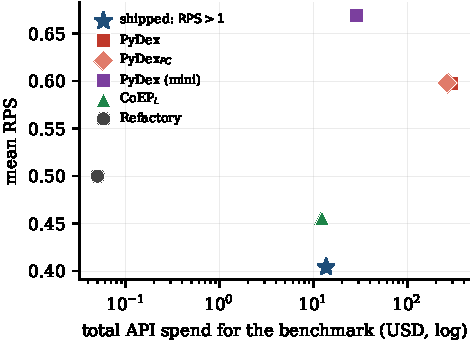
\includegraphics[width=\columnwidth]{../figures/fig_gate.pdf}
\caption{Mean RPS against total spend. Each small marker is one threshold
setting; the star is the shipped rule. Repair rate is identical across all of
them.}
\label{fig:gate}
\end{figure}

\section{What the Builder Writes}

\textbf{Three levels of generality.} What the builder writes is not one kind of thing, and the level predicts how far a rule travels. The most general level catches a language slip. \texttt{add\_missing\_call\_parens} describes itself as ``\texttt{x.pop} / \texttt{x.reverse} used as a statement or return value without \texttt{()}'', a Python trap that belongs to no assignment; it is the only one of the 128 builder-written rules that ever fired to do so on two assignments, repairing 8 submissions across R3 and C2. The middle level catches the misconception of one problem. \texttt{slice\_case\_check\_to\_equality} explains that ``\texttt{slice.isupper()} fails on empty slices (single char words)'' and repairs 108 submissions on C2, most of that assignment's rule-produced repairs; it cannot move to another problem but it would work for any class given this one. The most specific level is tied to the problem statement itself: \texttt{carry\_fix\_two\_value\_print} inserts an inch-to-foot carry check before the final print, fixing what it calls the ``compute feet first, round remainder second'' misconception, and repairs 28 of C4's 38 submissions on its own. That the authored layer is assignment-specific is therefore not a defect but a consequence of level. A rule that covers a class is written at the level of that class's misconception and so cannot cross assignments; a rule that crosses assignments does so because it knows nothing about the assignment.

% [번역] 부산물로 얻는 오개념 프로파일. 규칙이 만든 모든 패치는 그것을 만든 규칙 이름을 지니므로, 학급 단위로 집계하면 교수자가 읽을 수 있는 보고서가 된다. R2에서 규칙이 수리한 145건은 다음과 같이 갈린다. count_compare_relax 112건, undefined_domain_var_rename 28건, missing_return_false_append 22건, month_day_index_fix 7건이다. 이는 패치 목록이 아니라 이름 붙은 실수의 도수분포이며, 학급의 3분의 2가 같은 비교 오류를 냈다는 사실을 교수자에게 곧바로 말해 준다. 이 보고서는 수리의 부산물로 추가 비용 없이 나오고, 제출물당 API는 어떤 가격으로도 이를 방출하지 않는다. 호출은 패치를 낳지만 이름을 남기지 않기 때문이다.


% [번역] 규칙은 세 층위로 나뉜다. 빌더가 무엇을 쓰는지 보면 규칙이 하나의 종류가 아니라 일반성의 세 층위로 갈리고, 그 층위가 재사용 범위를 결정한다. 가장 일반적인 층은 언어 차원의 실수를 잡는다. add_missing_call_parens는 스스로를 "x.pop이나 x.reverse가 괄호 없이 문장이나 반환값으로 쓰였다"고 설명하는데, 이는 어떤 과제에도 없는 파이썬 자체의 함정이다. 빌더가 쓴 128개 규칙 중 두 과제 이상에서 발화한 유일한 규칙이 이것이고 R3과 C2에서 10건을 수리했다. 중간 층은 그 문제의 오개념을 잡는다. slice_case_check_to_equality는 "slice.isupper()가 한 글자 단어의 빈 슬라이스에서 실패한다"고 설명하며 C2에서 115건, 즉 그 과제 규칙 수리의 대부분을 처리한다. 다른 과제로 옮길 수는 없지만 이 과제를 낸 어느 학급에서나 통한다. 가장 특화된 층은 문제 서술 자체에 묶인다. carry_fix_two_value_print는 "인치가 12가 될 수 있는 '피트를 먼저 계산하고 나머지를 나중에 반올림하는' 오개념"을 고치려 최종 출력 앞에 인치→피트 올림 검사를 넣으며, C4의 38건 중 27건을 혼자 수리한다. 이 규칙은 다른 과제에서 의미가 없다. 따라서 작성 층이 과제 전용이라는 것은 결함이 아니라 층위의 함수다. 학급을 덮는 규칙은 그 학급의 오개념 수준에서 쓰이기 때문에 과제를 넘지 못하고, 과제를 넘는 규칙은 애초에 과제에 대해 아무것도 모르기 때문에 넘는다.
\textbf{A misconception profile falls out of repairing.} Every rule-produced patch carries the name of the rule that produced it, so aggregating over a class yields a report an instructor can read. On R2, of the 145 submissions the rules repaired under \texttt{claude-sonnet-5}, \texttt{count\_compare\_relax} accounts for 58, \texttt{undefined\_domain\_var\_rename} 27, \texttt{missing\_return\_false\_append} 22, and \texttt{month\_day\_index\_fix} 7, with the always-on comparison flip taking 33; a repair may compose rules, so these overlap. That is not a list of patches but a frequency table of named mistakes, and it says at once that one relaxed comparison accounts for 40\% of everything the rules repaired on this assignment. The report costs nothing beyond the repairing, and a per-submission API emits none of it at any price, because a call yields a patch but leaves no name behind.


\section{Self-Learning}

\begin{figure}[h]
\centering
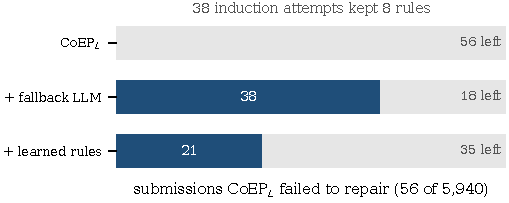
\includegraphics[width=\columnwidth]{../figures/fig_learn.pdf}
\caption{Self-learning, from the frozen tool's failures to the repairs its new
rules produce.}
\label{fig:learn}
\end{figure}

\section{Rule Provenance}

Table~\ref{tab:rules} lists the rules that carry the most submissions, counted
as distinct submissions rather than as applications, since a repair may compose
several rules. The distinction that matters is reuse: of the 128 rules the
builders wrote and that fired, exactly one fired on more than one assignment,
\texttt{add\_missing\_call\_parens}, which describes a Python trap rather than
anything about a problem. The always-on rules recur everywhere by construction,
which is why the builder's layer is priced per assignment and they are not.

\begin{table}[h]
\centering\scriptsize\setlength{\tabcolsep}{3pt}
\resizebox{\columnwidth}{!}{\begin{tabular}{llrr}
\toprule
Rule & where & submissions & assignments \\
\midrule
\texttt{generic\_flip\_compare} & always-on & 263 & 10 \\
\texttt{append\_missing\_return\_len\_after\_loop} & R1 & 114 & 1 \\
\texttt{slice\_case\_check\_to\_equality} & C2 & 108 & 1 \\
\texttt{generic\_shift\_index} & always-on & 74 & 5 \\
\texttt{strict\_one\_should\_be\_exactly\_one} & R2 & 70 & 1 \\
\texttt{count\_compare\_relax} & R2 & 58 & 1 \\
\texttt{generic\_shift\_range} & always-on & 50 & 7 \\
\texttt{capitalize\_title\_to\_swapcase} & C2 & 43 & 1 \\
\midrule
\multicolumn{4}{l}{128 builder-written rules fired, 1 on more than one assignment} \\
\bottomrule
\end{tabular}
}
\caption{The eight rules repairing the most submissions.}
\label{tab:rules}
\end{table}

\begingroup\sloppy
The eight rules self-learning absorbed read as misconceptions in the same way.
On R2 with \texttt{claude-sonnet-5}: \texttt{counter\_var\_confusion},
\texttt{uniqueness\_\allowbreak count\_gt1\_to\_neq1},
\texttt{index\_vs\_count\_\allowbreak and\_uncalled\_bool},
\texttt{missing\_else\_false}. On R2 with \texttt{gpt-5.4-mini}:
\texttt{count\_equality\_for\_uniqueness},
\texttt{count\_uniqueness\_\allowbreak instead\_of\_\allowbreak direct\_membership},
\texttt{missing\_call\_\allowbreak and\_predicate\_fix}. On C3:
\texttt{binarysearch\_zero\_exit}.
\endgroup

\section{Reproducibility}

The repository contains the harness, every prompt, the 22 synthesized
repairers with their build costs, and the per-submission event log each arm
wrote. Four commands regenerate every number in both documents from those logs
without touching a model: \texttt{run.py tables}, \texttt{run.py figures},
\texttt{run.py numbers}, which recomputes each quantity and reports whether the
string still occurs in the paper, and \texttt{run.py stats}. The measured
threshold settings are archived as \texttt{results/threshold\_sweep.json}.

Two dependencies are outside our control and worth stating. Both builders are
closed commodity models reached through their providers' APIs, so a rebuild
cannot be guaranteed to reproduce the same rules; what is released is the tools
those builds produced, which are ordinary Python and run offline. Refactory's
replication package is its authors' and is cloned rather than vendored.

\end{document}
